A sujeira acumulada ao longo do dia nem sempre necessita de uma limpeza profunda, uma simples
passada de vassoura ou um aspirador de pó resolve o problema. Porém muitas vezes há pouca
disposição para executar esta tarefa ou até mesmo falta de tempo. Para evitar o acumulo de
poeira, manter o ambiente limpo e sem a interferência humana, será desenvolvido um mecanismo 
autônomo capaz de aspirar as impurezas: o R2-PI2. O equipamento será composto de um robô móvel que realizará a aspiração e uma base fixa. O robô voltará para a base quando a bateria estiver acabando o que permite que o usuário não tenha a necessidade de carregá-lo manualmente. O objetivo do aspirador robô é garantir a limpeza do ambiente de forma automática com o mínimo de interação com o usuário.

\section{Problema Geral} % (fold)
\label{sub:problemaGeral}

Para a melhor compreensão do desenvolvimento do R2-PI2, foi elicitado com a equipe de desenvolvimento um problema principal que o robô irá solucionar. A tabela a seguir demonstra a descrição deste problema.

\begin{table}[H]
	\centering
	\caption{Descrição do Problema}
	\label{tab:equipe}
	\begin{tabular}{|c|c|c|}
	\hline
	\textbf{O problema de}      &  Sujeira acumulada nos cômodos da casa \\ \hline
	\textbf{Afeta}              &  Residentes da moradia sem tempo pra limpezas\\ \hline
	\textbf{Cujo impacto é}     &  Problemas de respiração e de saúde \\ \hline
	\textbf{Uma solução seria} 	&  Um aspirador de pó automatizado \\ \hline
	\end{tabular}
	\end{table}

% subsection subsection_name (end)

\subsection{Problemas Específicos} % (fold)
\label{sub:problemas_específicos}

Para um melhor entendimento do problema, foram identificados os seguintes problemas específicos:

\begin{itemize}
	\item Tempo perdido em limpeza da casa.
	\item Tempo perdido em remover os móveis para que o aspirador passe em todos os lugares.
	\item Carregar as baterias do aspirador de pó.
	\item Estar em casa para realizar a limpeza.
\end{itemize}

% subsection problemas_específicos (end)



\subsection{Pesquisa de Mercado} % (fold)
\label{sub:pesquisa_de_mercado}

	Atualmente, já existem outros robôs que também fazem limpeza automatizada. Para fins de pesquisa de mercado, foram encontrados os seguintes robôs \cite{techtudo}:

	\begin{itemize}
		\item \textbf{Aspirador de Pó Compacto Home UP:}

			O aspirador de pó inteligente tem um design compacto que permite entrar embaixo de sofás e camas, para remover a poeira. A opção tem armazenamento de até 400 ml com saco coletor e oferece escovas laterais. O aparelho funciona por bateria recarregável e está disponível na cor preto. A garantia do fornecedor é de 6 meses e ele tem dimensões de 400 x 345 x 135 mm, com peso de 2 Kg. O preço fica em torno de R\$ 819 em lojas online nacionais.

			\begin{figure}[H]
				\centering
				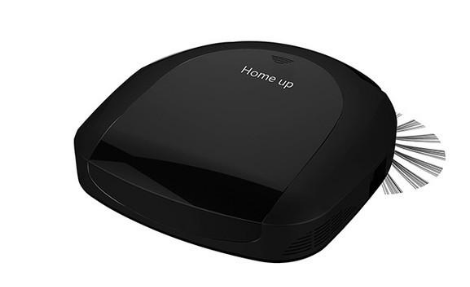
\includegraphics[scale=0.55]{figuras/pm_home_up.png}
				\caption{Aspirador de Pó Compacto Home UP.}
				\label{img:pm_home_up}
			\end{figure}

		\item \textbf{Aspirador de pó Ecovacs Beebot D35:}

			 O modelo da Ecovacs é equipado com sensores para evitar quedas ou bater em objetos, por exemplo. O aspirador de pó tem filtro bactericida e há uma bateria interna que dura cerca de 1 hora. É possível programar para fazer uma limpeza automática durante o dia e a garantia é de 1 ano. O design compacto permite entrar em espaços com 6 cm de altura e nas dimensões ele tem 300 x 290 x 50 mm, com peso de 2,2 kg. O aspirador robô pode ser comprado com preço a partir de R\$ 954.

			\begin{figure}[H]
				\centering
				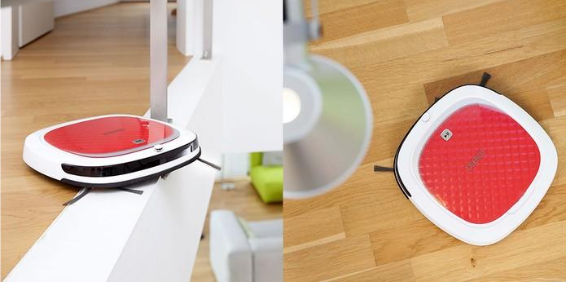
\includegraphics[scale=0.55]{figuras/pm_beebot_d35.png}
				\caption{Aspirador de pó Ecovacs Beebot D35.}
				\label{img:pm_beebot_d35}
			\end{figure}


		\item \textbf{Aspirador de Pó robô Fun Clean:}

			 O aspirador inteligente da Fun Clean tem funções programáveis para limpeza automática, é equipado com controle remoto, sensores para evitar quedas e bateria recarregável na base. O design circular na cor vermelha oferece luzes e tem funcionamento bivolt. A garantia é de 3 meses e nas dimensões estão 340 x 340 x 90 mm, com peso de 2,8 kg. Sobre o preço, o aparelho pode ser encontrado a partir de R\$ 991 em lojas online nacionais.

			\begin{figure}[H]
				\centering
				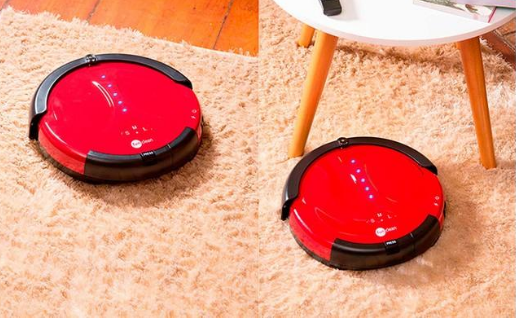
\includegraphics[scale=0.55]{figuras/pm_fun_clean.png}
				\caption{Aspirador de Pó robô Fun Clean.}
				\label{img:pm_fun_clean}
			\end{figure}

		\item \textbf{Aspirador de Pó Ropo Glass:}

			A opção da Ropo Glass também oferece funções smarts para ajudar na limpeza da casa. Está disponível controle remoto e limpeza programável, podendo ser usado em diferentes tipos de piso como madeira, cerâmicos e até carpetes. Por dentro está uma bateria recarregável que dura cerca de 2 horas, lâmpada UV de esterilização, painel touch iluminado e sensores para evitar batidas e quedas. Nas medidas estão 500 x 320 x 160 mm com peso de 3,1 kg. A garantia é de 6 meses e o preço a partir de R\$ 1.393 em lojas online na cor preto.

			\begin{figure}[H]
				\centering
				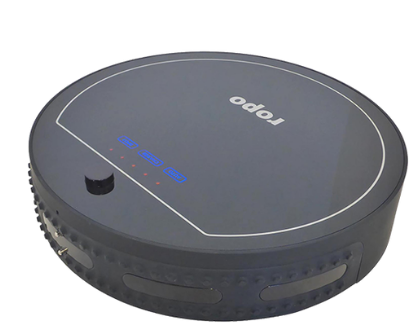
\includegraphics[scale=0.55]{figuras/pm_ropo_glass.png}
				\caption{Aspirador de Pó Ropo Glass.}
				\label{img:pm_ropo_glass}
			\end{figure}

		\item \textbf{Aspirador de pó robô Deboot 4:}

			Com uma configuração mais completa, o modelo Deboot 4 da Ecovacs tem função dupla de limpeza à vácuo e permite aspirar, varrer e até passar pano no piso da casa, com ações simultâneas. Por dentro está uma bateria recarregável e permite limpar embaixo os móveis ou nos cantos, com luzes indicadoras no painel. As funções programáveis permitem fazer limpezas automáticas, oferece sensores anti-choque e tem funcionamento por controle remoto. O preço é de R\$ 1.399 em lojas virtuais brasileiras.

			\begin{figure}[H]
				\centering
				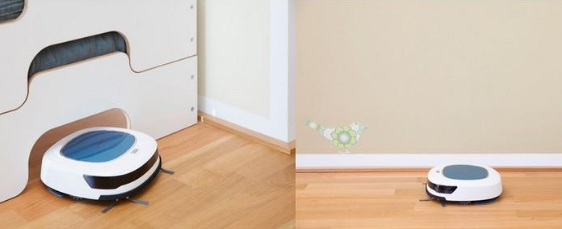
\includegraphics[scale=0.55]{figuras/pm_deboot_4.png}
				\caption{Aspirador de pó robô Deboot 4.}
				\label{img:pm_deboot_4}
			\end{figure}

		\item \textbf{Aspirador de pó Ecovacs D63:}

			O modelo D63 da Ecovacs vem recursos extras no aspirador de pó inteligente, com filtro antibactericida e detectores inteligentes de poeira e anti-choque. O usuário consegue programas horário da limpeza e tem quatro modos automáticos, para todo o local, ambientes específicos ou cantos. Permite uso em piso de madeira cerâmica, mármore e carpete, com dimensões de 340 x 340 x 100 mm e peso de 2,7 kg.  O modelo tem preço a partir de R\$ 1.872 em lojas online.

			\begin{figure}[H]
				\centering
				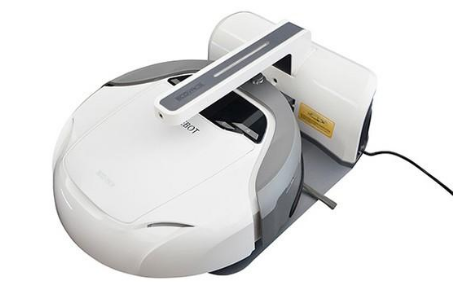
\includegraphics[scale=0.55]{figuras/pm_ecovacs_d63.png}
				\caption{Aspirador de pó Ecovacs D63.}
				\label{img:pm_ecovacs_d63}
			\end{figure}

		\item \textbf{Aspirador Roomba 620 iRobot:}

			O modelo iRobot da Roomba pemite ajustar funções smart e faz a limpeza em três etapas, de forma mais completa. A tecnologia AeroVac ajuda a recolher os resíduos durante o uso e a bateria dura cerca de 90 minutos. Estão disponíveis sensores para detectar poeira, o design tem laterais macias para não arranhar os móveis, além de identificar escadas. O aparelho pode ser usado em pisos de madeira, cerâmica e até carpetes. O tamanho é de 330,2 x 330,2 x 128 mm com peso de 3,6 kg e garantia de 12 meses. O preço fica em torno de R\$. 2.099 no Brasil, no modelo de cor branca.

			\begin{figure}[H]
				\centering
				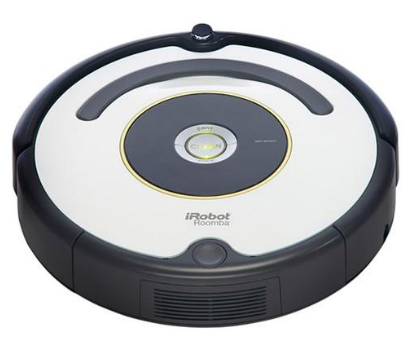
\includegraphics[scale=0.55]{figuras/pm_roomba.png}
				\caption{Aspirador Roomba 620 iRobot.}
				\label{img:pm_roomba}
			\end{figure}

	\end{itemize}

% subsection pesquisa_de_mercado (end)



\section{Proposta} % (fold)
\label{sub:proposta}
	
	O objetivo geral desse projeto é proporcionar ao usuário/cliente a oportunidade de limpar sua casa de forma cômoda e confortável para o mesmo. Este objetivo será alcançado através da remoção da poeira e/ou partículas de sujeira encontradas no cômodo da casa. A solução proposta neste projeto será a criação de um robô aspirador autônomo, que auxiliará na tarefa supracitada. 

	Tal robô terá capacidade de desviar os obstáculos encontrados durante seu percurso, além de ter autonomia de voltar à sua base quando necessário (ao término da tarefa ou quando sua bateria estiver prestes a acabar), a fim de se carregar.

	Esta solução está organizada segundo a EAP (Estrutura analítica do projeto) apresentada na Figura \ref{img:eap}, destacando os entregáveis e seus subsistemas ao longo de todo o projeto.
	
	\begin{figure}[H]
		\centering
		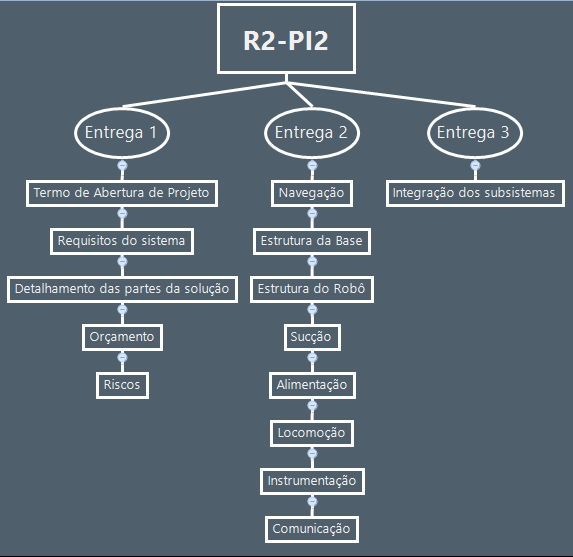
\includegraphics[scale=0.55]{figuras/eap.png}
		\caption{Estrutura Analítica do Projeto do R2-PI2.}
		\label{img:eap}
	\end{figure}

	A primeira entrega consiste basicamente do gerenciamento do projeto. Está etapa é de suma importância para o desenvolvimento do projeto, visto que nela será definida a solução para o problema exposto, bem como os requisitos necessários para garantir o êxito na conclusão do projeto. Analisando a EAP fica evidente como foi feita a separação dos subsistemas do produto final. O desmembramento das entregas facilita a realização de atividades ao longo do projeto. Vale ressaltar que mesmo produzidos separadamente os subsistemas devem se desenvolver em total harmonia, a fim de alcançar o objetivo final.

% subsection proposta (end)



\section{Objetivo Geral} % (fold)
\label{sub:objetivo_geral}
	
	Algumas pessoas costumam limpar suas residências de forma regular e outras que por motivos diversos só fazem isso esporadicamente. O desenvolvimento do R2-PI2 tem como alvo atender aos usuários que desejam manter o local limpo de modo automático e com o mínimo de intervenção humana. Alguns aspiradores robôs já fazem a limpeza do ambiente automaticamente, porém uma parcela deles necessita que o usuário tenha que procurá-los pela casa enquanto eles emitem um sinal sonoro indicando que a bateria está quase descarregada. O R2-PI2 será apto a voltar sozinho para a base e permanecer lá até que a bateria seja carregada, além de manter-se inativo na base ele poderá voltar a efetuar a higienização do local quando programado pelo utilizador. Outros objetivos que devem ser atendidos pelo dispositivo aspirador, estão listados no item seguinte.

% subsection objetivo_geral (end)

\subsection{Objetivos Específicos} % (fold)
\label{sub:objetivos_específicos}
	
	\begin{itemize}
		\item Controle a distância;
		\item Se locomover pelo cômodo e desviar de obstáculos;
		\item Comunicação entre o Robô e a central de processamento;
		\item Identificar e sinalizar status da bateria;
		\item Possuir sistema de acompanhamento do status do robô
		\item Conter acionamento de start/stop;
		\item Gerar relatório de atividades;
		\item Sistema de agendamento de limpezas.
	\end{itemize}
% subsection objetivos_específicos (end)


\section{Equipe e Responsabilidades} % (fold)
\label{sub:equipe_e_responsabilidades}

	A equipe do projeto está distribuida de acordo com a Tabela \ref{tab:equipe}. Ou seja, é uma equipe formada por 14 (catorze) estudantes, distribuidos em 5 (cinco) engenharias distintas, o que torna a gestão e distribuição do conhecimento uma tarefa bastante complicada.

	\begin{table}[H]
	\centering
	\caption{Equipe do projeto R2-PI2}
	\label{tab:equipe}
	\begin{tabular}{|c|c|c|}
	\hline
	\textbf{Nome}                              & \textbf{Matricula} & \textbf{Engenharia} \\ \hline
	Kaio Diego de Araujo Coelho                & 12/0123673         & Eletrônica          \\ \hline
	Laryssa Lorrany Olinda Costa               & 12/0060973         & Eletrônica          \\ \hline
	Mônica Damasceno Cavalcante Castelo Branco & 10/0037097         & Eletrônica          \\ \hline
	Rafael Fazzolino Pinto Barbosa             & 11/0136942         & Software            \\ \hline
	Ricardo Gonçalves Teixeira                 & 12/0021561         & Software            \\ \hline
	João Paulo Siqueira Ribeiro                & 12/0014378         & Software            \\ \hline
	Thais Soares Monteiro                      & 11/0066561         & Energia             \\ \hline
	Pedro Henrique de Queiroz Rocha            & 11/0083890         & Energia             \\ \hline
	Jair Jorge Medeiros                        & 11/0013760         & Energia             \\ \hline
	Hildoglas Botelho Chaves                   & 11/0121104         & Energia             \\ \hline
	Luan de Oliveira Noleto                    & 11/0128419         & Energia             \\ \hline
	Rafael de Souza Freitas                    & 11/0019300         & Automotiva          \\ \hline
	Yago Henrique Melho Honda                  & 12/0042840         & Aeroespacial        \\ \hline
	Márcia Aline Ribeiro Silva                 & 12/0017806         & Aeroespacial        \\ \hline
	\end{tabular}
	\end{table}

	Como estamos trabalhando com áreas de conhecimento distintas, vê-se a necessidade de buscar maneiras que possam garantir maior equilíbrio de conhecimento na equipe, seja relacionado ao processo de desenvolvimento ou à áreas específicas de cada sub-sistema. Com este objetivo, adotamos o papel de \textit{Scrum master} como um facilitador durante as \textit{sprints} de desenvolvimento.

	Entretanto, a simples adoção deste papel pode não garantir a distribuição do conhecimento pela equipe, desse modo optou-se por rotacionar o papel de \textit{scrum master} entre os integrantes. Fazendo com que cada integrante tenha a oportunidade de vivenciar esta experiência pelo período de uma \textit{sprint}, ou seja, 2 (duas) semanas.

	A distribuição das responsabilidades em relação ao desenvolvimento da solução estão de acordo com a Tabela \ref{tab:areas}, onde estão destacados os sub-sistemas presentes na solução.

	% Please add the following required packages to your document preamble:
% \usepackage{multirow}
\begin{table}[H]
\centering
\caption{Equipe - Áreas de atuação}
\label{tab:areas}
\begin{tabular}{|c|c|}

\hline
\multirow{2}{*}{\textbf{Eletrônica}}                                                            & Sensoriamento               \\ \cline{2-2} 
                                                                                                & \multirow{2}{*}{Comunicação} \\ \cline{1-1}
\multirow{3}{*}{\textbf{Software}}                                                              &                              \\ \cline{2-2} 
                                                                                                & Navegação                    \\ \cline{2-2} 
                                                                                                & Interface                    \\ \hline
\textbf{Energia}                                                                                & Alimentação                  \\ \hline
\multirow{3}{*}{\textbf{\begin{tabular}[c]{@{}c@{}}Automotiva\\ e\\ Aeroespacial\end{tabular}}} & Estrutura                    \\ \cline{2-2} 
                                                                                                & Locomoção                    \\ \cline{2-2} 
                                                                                                & Sucção                       \\ \hline
\end{tabular}
\end{table}

% subsection equipe_e_responsabilidades (end)
\subsection{Política de Comunicação da Equipe} % (fold)
\label{sub:política_de_comunicação_da_equipe}
	
	Para a comunicação do grupo foram escolhidas algumas ferramentas de comunicação para facilitar a organização do grupo. De maneira informal foi adotado o aplicativo \textit{Whatsapp}. Como foi adotado o \textit{Scrum}, para o gerenciamento do projeto, está sendo utilizado o \textit{Trello}\footnote{www.trello.com} para organizar todas as atividades a serem feitas e registrar as que já estão prontas, utilizando a técnica de Kanban. Para compartilhar e editar documentos para os pontos de controle foi criada uma pasta no \textit{Google Drive}\footnote{www.drive.google.com}. 

	A última ferramenta para a comunicação do grupo é a plataforma \textit{Slack}\footnote{www.slack.com}, que funciona como um chat, podendo criar canais de comunicação que apenas os interessados no assunto entram no canal facilitando a troca de informações sobre determinado assunto ou sobre determinada parte do projeto. Além do canal geral com todos os integrantes onde ocorre a discussão com o grupo todo, um canal criado no \textit{Slack} e bastante importante é o \textit{daily}, onde cada um deve, diariamente, descrever o que fez no dia para o Projeto, para facilitar o controle do grupo. 


% subsection política_de_comunicação_da_equipe (end)
\subsection{Organização do Trabalho} % (fold)
\label{sub:organização_do_trabalho}
	
	Este trabalho está organizado de maneira a apresentar as sub divisões presentes no projeto, basicamente dividindo o sistema geral em diversos sub-sistemas independentes, que ao fim do projeto poderão ser integrados para o funcionamento ideal da solução. A solução está apresentada no capítulo \ref{cha:solucao}, sub-dividida nas seções \ref{sub:requisitos_do_sistema}, onde são apresentados os requisitos do trabalho, \ref{sub:alimentação}, onde está apresentada a solução referente a sustentação energética do projeto, \ref{sub:automação}, onde são descritos os detalhes de navegação do robô, \ref{sub:locomocao}, onde são detalhadas as características da estrutura do robô e seu sistema de locomoção, \ref{sec:estrutura_da_base}, onde se encontram os detalhes referentes a estrutura da base, \ref{sub:aspirador}, o sistema de sucção, \ref{sub:instrumentação}, onde estão detalhados os sensores utilizados, \ref{sub:Hardwar_para_Comunicação}, onde se encontra o \textit{hardware} para comunicação, \ref{sub:controle}, onde se encontra a solução relacionada ao controle do sistema, \ref{sub:comunicação}, possuindo a solução de comunicação do sistema e \ref{sub:interface}, possuindo os detalhes da interface do usuário.

	Após a apresentação de toda a solução do projeto, é apresentado o plano de gerenciamento de riscos do projeto, na seção \ref{cha:riscos}. Ao fim, é apresentado o processo de desenvolvimento do projeto, assim como a metodologia adotada pela equipe, na seção \ref{cha:metodologia}.
% subsection organização_do_trabalho (end)
